\documentclass{article}
\usepackage[utf8]{inputenc}
\usepackage[utf8]{inputenc}
\usepackage{eucal}
\usepackage[utf8]{inputenc}
\usepackage{amsfonts, amssymb, amsmath}
\usepackage{graphicx}

\title{Reti di calcolatori}
\author{kocierik }
\date{September 2021}

\begin{document}

\tableofcontents

\maketitle

\section{Rete di calcolatori}
Una rete di calcolatori è un insieme di dispositivi autonomi e interconnessi
Utilizzata per condividere risorse, accessi remoti...

\subsection{Classificazione reti}
\begin{itemize}
    \item \textbf{PAN} Persona Area Network
    \item \textbf{LAN} Local Area Network
    \item \textbf{MAN} Metropolitana Area Network
    \item \textbf{WAN} Wide Area Network
    \item \textbf{Internet} rete globale
\end{itemize}

\subsubsection{Prestazioni}
L'\textbf{indice nominale massimo} indica la massima velocità raggiungibile.
Le prestazioni delle reti di calcolatori vengono misurate attraverso:
\begin{itemize}
    \item \textbf{Capacità di trasmissione}: (numero di bit o in byte)
    \item \textbf{Ritardo del collegamento}: tempo richiesto ai dati per transitare da mittente a destinatario
\end{itemize}
Il \textbf{jitter} indica di variazione del ritardo di rete di una o più caratteristiche di un segnale. Differenza di tempo tra i pacchetti inviati.

\subsection{Componenti}
\begin{itemize}
    \item \textbf{Scheda di rete}, codifica e trasmette i dati (driver necessari API)
    \item \textbf{Mezzo di trasmissione}, supporto fisico (doppini,fibra)
    \item \textbf{Connettore di rete}, interfaccia per il collegamento del dispositivo, \textbf{RJ-45} (cavo ethernet).
    \item \textbf{Protocolli di rete}, regole da rispettare per garantire compatibilità tra dispositivi
\end{itemize}

\textbf{gabbia di Faraday} si intende qualunque sistema conduttore in grado d'isolare l'ambiente interno da un qualunque campo elettrostatico.\\
 \textbf{PCI} = Peripheral Component Interconnect

\subsection{Collegamenti e infrastrutture di rete}
\begin{itemize}
    \item \textbf{Connesione o collegamento di rete}
    \begin{itemize}
        \item nodi
        \item host
    \end{itemize}
    \item \textbf{Infrastruttura di rete}, struttura di rete a connesioni multiple:
    \begin{itemize}
        \item Completamente connesse (ogni nodo è raggiungibile in un passo)
        \item Parzialmente connesse ( connessione coperta solo da un singolo percorso)
        \item Partizioi di rete (gruppo di componenti isolato da altri
    \end{itemize}
    \item \textbf{Cammino dei segnali}, diretto o indiretto attraverso connessioni in sequenza
\end{itemize}

\subsection{Topologia di rete}
Le infrastrutture di rete possono avere diverse tipologie: 
\begin{itemize}
    \item Anello
    \item Stella (più utilizzata)
    \item Bus
    \item Albero
\end{itemize}

\begin{center}
    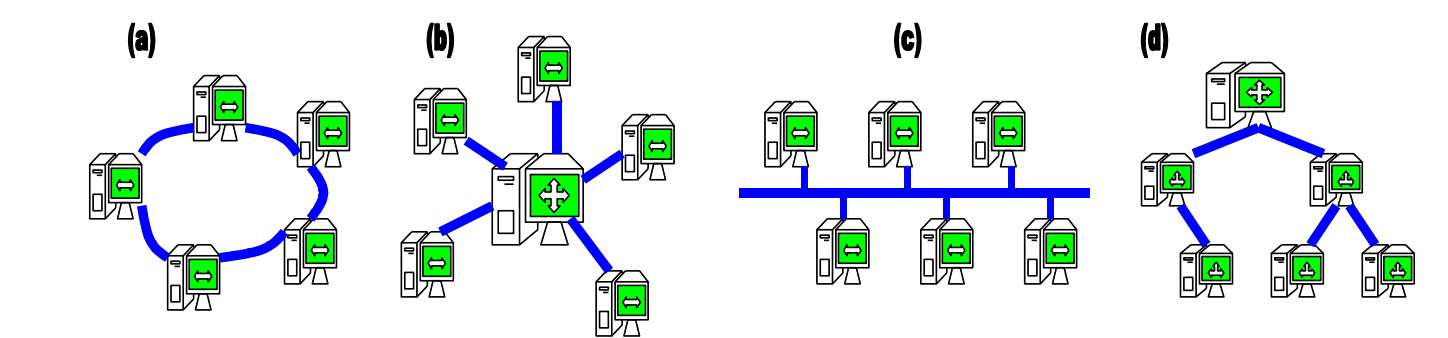
\includegraphics[width=10cm]{img/topologie.png}
\end{center}
Reti più grandi possono avere una topologia a \textbf{maglia}.

\subsection{Mezzo di trasmissione}
Il \textbf{mezzo di trasmissione} usato per la connessione fisica può essere di tre tipi:
\begin{itemize}
    \item \textbf{Cavetti o fili metallici}, trasmettono segnali elettrici
    \item \textbf{Fibre ottiche}, trasmettono segnali luminosi
    \item \textbf{Senza fili (Wireless)}, trasmettono radiazioni elettromagnetiche
\end{itemize}

\subsection{Scheda di rete}
La scheda di rete è un componente dotato di:
\begin{itemize}
    \item Interfaccia di collegamento
    \item Un connettore di rete
\end{itemize}
Esso trasmette e riceve i dati, codificandoli e decodificandoli:
\begin{itemize}
    \item Dal calcolatore al mezzo di trasmissione
    \item Dal mezzo di trasmissione al calcolatore
\end{itemize}
Dipende inoltre dal mezzo di trasmissione
\begin{itemize}
    \item Scheda di rete per mezzi disici cablati, ottici, wireless
\end{itemize}
Ha un codice identificativo univoco chiamato \textbf{MAC} (medium access control)\\
\textbf{Broadcast:} Un computer collegato a una rete invia un pacchetto dati simultaneamente a tutti gli altri partecipanti della stessa rete.

\subsubsection{Canali di comunicazione della rete}
Il canale di comunicazione è la \textbf{virtualizzazione} del mezzo fisico di comunicazione. Un canale ad \textbf{accesso multiplo} invece, è un canale il quale tutti i dispositivi ricevono e trasmettono i dati.
\begin{itemize}
    \item Rischio di collisioni
    \item Richiedono indirizzamenti
\end{itemize}

\subsection{Reti a commutazione}
Le reti sono composti da una serie di canali in cascata, permettendo la comunicazione tra due dispositivi anche molto lontani. Vengono utilizzate due modalità principali:
\begin{itemize}
    \item \textbf{Commutazione a circuito} (linea telefonica). In questo modo:
    \begin{itemize}
        \item Viene riservato un circuito di canali di comunicazione punto a punto per ogni connessione
        \item Un \textbf{basso} utilizzo di \textbf{risorse} di rete (canale sprecato quando non si trasmette)
        \item Costo vario in base al tempo
        \item Ritardo di connessione basso
    \end{itemize}
    \item \textbf{Commutazione a pacchetto}, molto utilizzate in reti basate su canali ad accesso multiplo ( broadcast), ogni pacchetto è indipendente. In particolare, su canali ad accesso multiplo:
    \begin{itemize}
        \item Ogni pacchetto contiene l'indirizzo del destinatario
        \item Si ha condivisione del canale tra diversi flussi di pacchetti
        \item Minor numero di risorse
        \item Si paga per quantità di dati trasmessi
    \end{itemize}
\end{itemize}

\subsection{Servizi orientati alla connessione e non}
Nelle reti a \textbf{commutazione di pacchetto} il servizio di trasmissione ha proprietà determinate dal ruolo dei protocolli utilizzati

\begin{itemize}
    \item I dati sono spediti in pacchetti
    \item I pacchetti arrivano in ordine disordinato
    \end{itemize}
     Servizi \textbf{orientati alla connessione} (connection-oriented) (telefono)
    \begin{itemize}
        \item Garantisce la consegna ordinata dei pacchetti
        \item Garantisce la ri-trasmissione di eventuali pacchetti persi
    \end{itemize}
    Servizi \textbf{non orientati alla connessione} (connectionless), (lettere di posta ordinaria)
    \begin{itemize}
        \item I pacchetti possono seguire strade diverse, e arrivare in ordine diverso
    \end{itemize}


\subsection{Protocolli di rete organizzati a livello}

Gli aspetti di gestione della comunicazione nella rete è definita da:
\begin{itemize}
    \item Definizione di \textbf{protocollo:}
    \begin{itemize}
        \item Regole e procedure (semantiche) di gestione dei processi
        \item Regole e formati (sintattici)
        \item Permette compatibilità
    \end{itemize}
    \item \textbf{Architettura dei protocolli di rete:}
    \begin{itemize}
        \item Ogni livello affronta e risolve un problema della comunicazione
        \item I livelli superiori effettuano richieste di servizio
        \item I livelli inferiori fornisocno servizi al livello superiore
    \end{itemize}
\end{itemize}

\subsection{Architettura Standard di protocolli di rete}

Esiste un riferimento standard per definire l'architettura dei protocolli delle reti:
\begin{itemize}
    \item \textbf{Standard ISO/OSI RM} (Open System Interconnection Reference Model)
    \begin{itemize}
        \item Insieme di livelli completo e rigoroso
    \end{itemize}
    \item Definisce un'architettura dei protocolli in 7 livelli
    \begin{itemize}
        \item Ogni livello gestisce una classe di problematiche di rete
        \item Ogni livello fornisce ai livelli superiori una visione della rete semplificata
        \begin{itemize}
            \item Dialoghi tra livelli paritari
            \item Dialoghi tra livelli sovrapposti
        \end{itemize}
    \end{itemize}
\end{itemize}

\begin{center}
    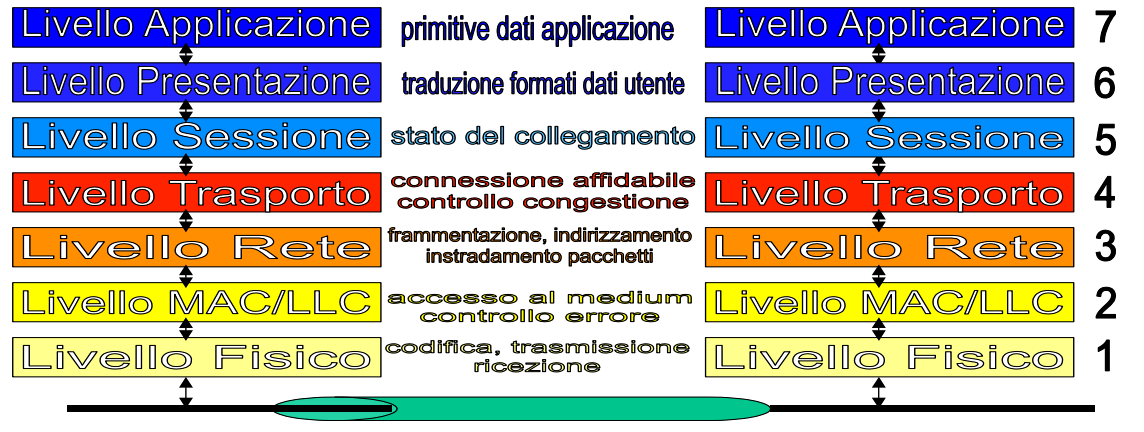
\includegraphics[width=10cm]{img/ISO:OSI.png}
\end{center}

L'architettura dei livelli di protocolli di internet utilizza solo   \textbf{5 dei 7 livelli ISO/OSI RM}:
\begin{itemize}
    \item Ogni livello comunica con quello adiacente passando il contenuto dei dati ottenuti:
    \begin{itemize}
        \item Il livello trasporto imbusta i pacchetti e controlla la velocità d'invio
        \item Il livello rete frammenta i dati in pacchetti, decidendo su quale cammino far percorrere
        \item Il livello MAC/LLC esegue la consegna finale dei dati
    \end{itemize}
\end{itemize}

\begin{center}
    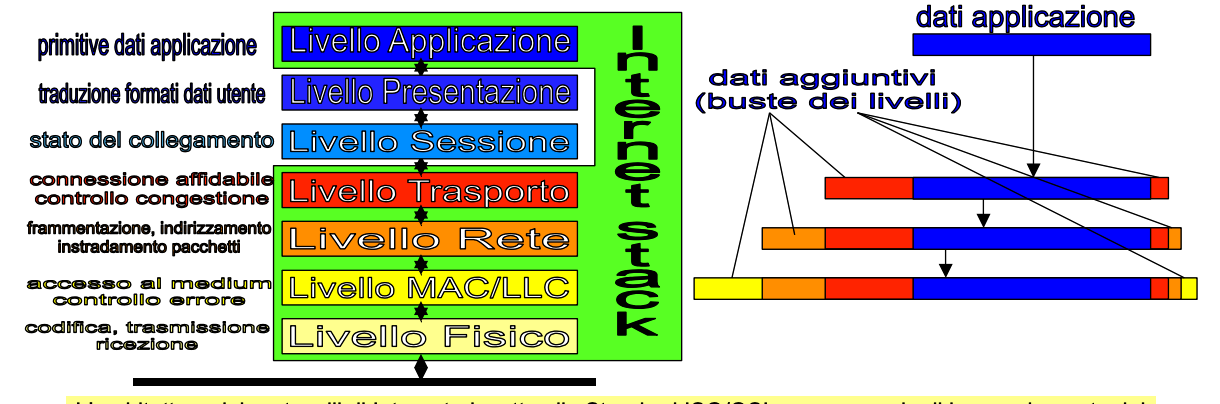
\includegraphics[width=10cm]{img/architettura2.png}
\end{center}

\subsection{Livelli e integrazione delle reti}

Ad ogni livello i protocolli gestisdcono problemi diversi e la rete assume caratteristiche di integrazione e proprietà diverse:
\begin{itemize}
    \item \textbf{Livello fisico,} la rete è solo un mezzo di trasmissione condiviso tra dispositivi
    \item \textbf{Livello MAC/LLC,} la rete è locale, esso regola gli indirizzo dei dispositivi, i tempi di accesso, e gestione degli errori
    \item \textbf{Livello rete}, la rete è una collezione di reti, e assume struttura gerarchica
    \begin{itemize}
        \item Regole per indirizzi di rete
        \item Si definiscono nuovi router che smistano i pacchetti
    \end{itemize}
    \item \textbf{Livello trasporto}, la rete è una collezione di reti organizzate gerarchicamente, regola la spedizione affidabile di pacchetti e controlla la congestione della rete
    \item \textbf{Livello applicazione}, la rete esiste, ed è utilizzabile dalle applicazioni dell'utente
\end{itemize}
\textbf{Dominio di collisione:} Gruppo di host collegato in modo che se due persone parlano contemporaneamente c'è collisione


\section{Livello fisico}
La trasmissione dati sul canale di comunicazione richiede la \textbf{codifica e decodifica dei dati} sul mezzo trasmissivo, da parte della scheda di rete.
\begin{itemize}
    \item \textbf{dati digitali bit}
    \item Codifica dei dati \textbf{digitali} usando segnali \textbf{analogici}
    \item Tutti i segnali viaggiano alla velocità della luce
    \item La capacità del canale di trasmissione: il valore massimo di bit/secondo trasmessi
\end{itemize}

\subsection{Segmento di rete locale}
\begin{itemize}
    \item Segmento di rete locale, un mezzo di trasmissione condiviso con canale ad accesso multiplo, tutte le schede di rete ricevono le trasmissioni
    \item ogni scheda di rete ha assegnato un indirizzo fisico diverso: \textbf{indirizzo MAC}
    \item compiti e servizi offerti dai protocolli di livello 2 (MAC/LLC): \textbf{accesso al mezzo trasmissivo}
    \begin{itemize}
        \item Trasmissione e indirizzamento del livello MAC
    \end{itemize}
\end{itemize}

\subsubsection{Come rendere il segmento affidabile}
Il livello 2 \textbf{(MAC/LLC)} deve verificare se il frame è stato ricevuto correttamente. Esso invia un \textbf{frame di conferma} della corretta ricezione al mittente. Se il mittente non riceve conferma entro un tempo fissato, trasmette di nuovo il \texttt{frame}. I tentativi di trasmissione vengono ripetuti finché non si ottiene la conferma del successo.
\begin{center}
    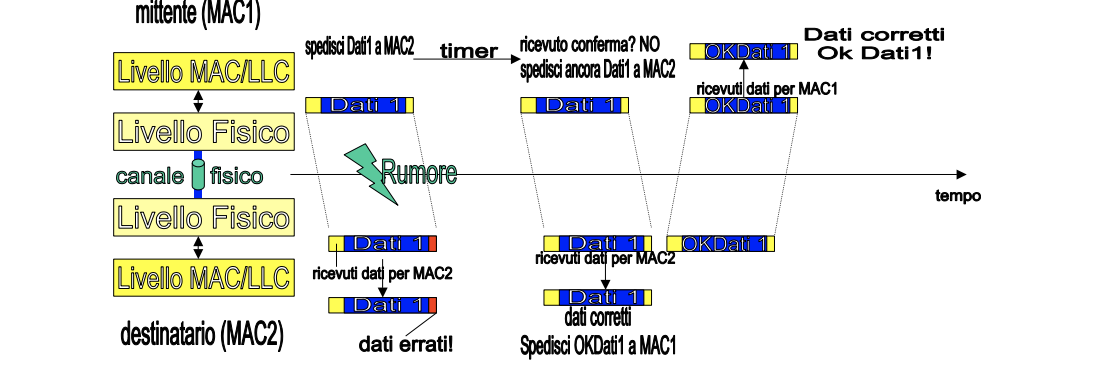
\includegraphics[width=10cm]{img/esFrame.png}
\end{center}
\begin{center}
    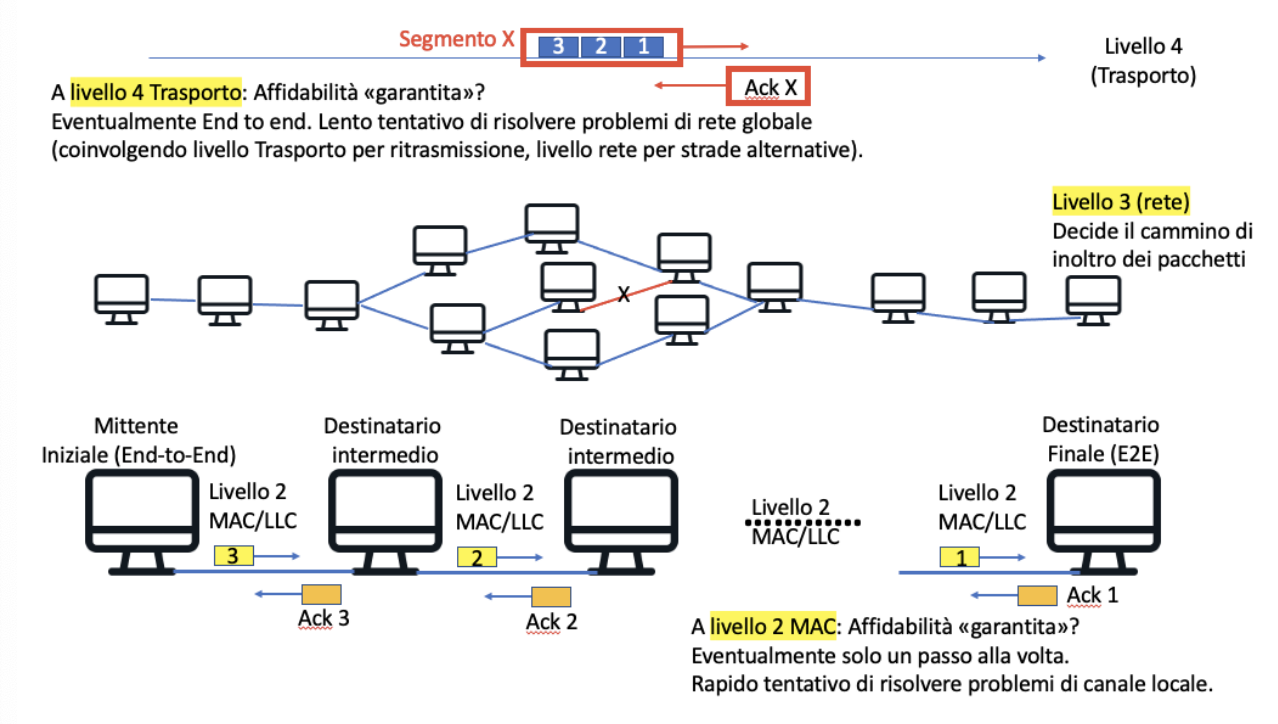
\includegraphics[width=10cm]{img/esFrame2.png}
\end{center}

\subsection{Tecnologie per schede di rete: 3 esempi}
Tre esempi di protocolli di livello due, che possono essere usati in alternativa tra loro per le schede di rete di segmenti di rete locale, sono:
\begin{itemize}
    \item \textbf{Ethernet}
    \begin{itemize}
        \item Molto usato in reti locali cablate
        \item La scheda di rete ascolta il canale e trasmette solo se nessuno sta già trasmettendo
        \item Se viene rilevata una collisione la trasmissione è interrotta per riprovare più tardi
    \end{itemize}
    \item \textbf{IEEE 802.11 (WI-FI)}
    \begin{itemize}
        \item E' alla base delle reti locali senza fili
        \item La scheda di rete ascolta il canale e trasmette solo se nessuno sta già trasmettendo
        \begin{itemize}
            \item Si cerca di prevenire le collisioni dilazionando le trasmissioni nel tempo
        \end{itemize}
    \end{itemize}
    \item \textbf{Token ring}
    \begin{itemize}
        \item Usata se i dispositivi sono collocati su topologia ad anello cablato
        \item Esiste un frame detto \textbf{token} che viene passato com un testimone tra i dispositivi
        \item Solo chi detiene il \textbf{token} ha diritto di trasmettere, poi deve passare il token
    \end{itemize}
\end{itemize}

\begin{center}
    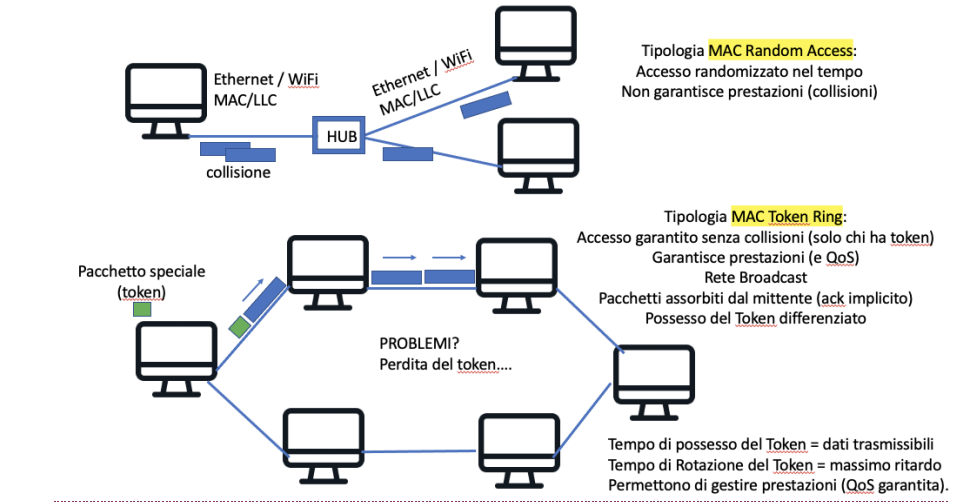
\includegraphics[width=10cm]{img/esrete.png}
\end{center}

\subsection{Comporre segmenti in rete locali}
Dispositivi utili a \textbf{comporre reti locali} di calcolatori, agendo al \textbf{livello fisico} e MAC/LLC:
\begin{itemize}
    \item \textbf{Repeater}, livello fisico:
    \begin{itemize}
        \item I segnali trasmessi sul mezzo fisico degradano la distanza
        \begin{itemize}
            \item Limite massimo alla lunghezza di un segnmento di rete Ethernet (100-200 metri)
        \end{itemize}
        \item Un \textbf{repeater} è un dispositivo che amplifica e rigenera il segnale ricevuto
        \begin{itemize}
            \item Collega due o più segmenti di rete
            \item Estende la lunghezaa dei segnali dei segmenti di rete locale
        \end{itemize}
    \end{itemize}
    \textbf{Hub}, livello fisico (detto anche \textbf{repeater}:
    \begin{itemize}
        \item Dispositivo concentrato e punto di contatto della connesione
    \end{itemize}
    \item \textbf{Bridge:}, livello MAC/LLC:
    \begin{itemize}
        \item Connette segmenti di una rete locale con tecnologie MAC diverse:
        \begin{itemize}
            \item Connette un segmento \textbf{Ethernet} a un segmento \textbf{Token Ring}
            \item Tradue i \textbf{frame} ricevuti da un segmento nel formato \item \textbf{frame} dell'altro segmento
            \item Ri-trasmette il frame tradotto usando il protocollo \textbf{MAC} opportuno
         \end{itemize}
    \end{itemize}
    \item \textbf{Switch}, livello MAC/LLC:
    \begin{itemize}
        \item Analogo al \textbf{bridge}, ma permetti di connettere molti segmenti (10-12)
        \item Ha capacità di filtrare e inviare i \textbf{frame} sul segmento giusto, leggendo l'indirizzo MAC del destinatario del frame
    \end{itemize}
\end{itemize}
\begin{center}
    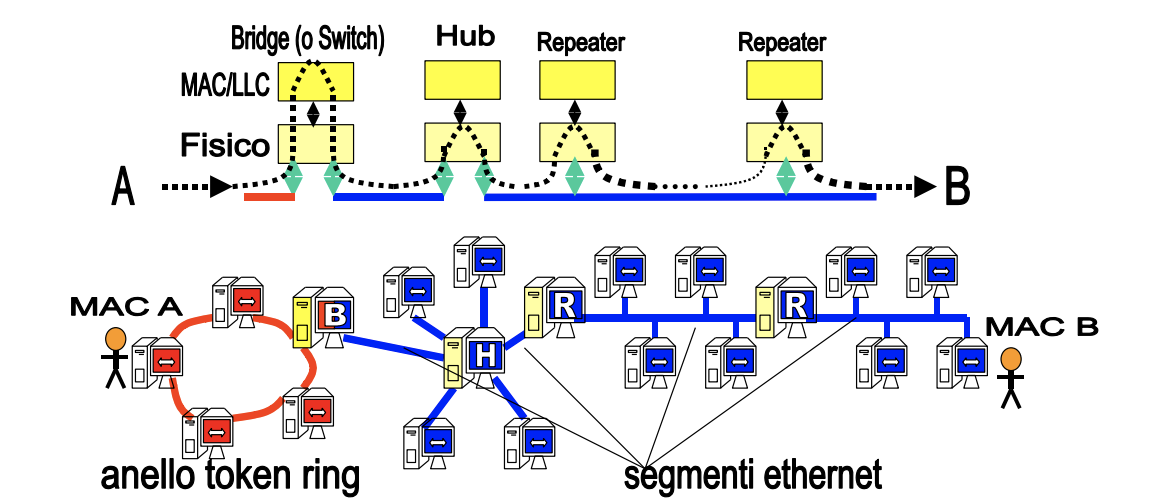
\includegraphics[width=10cm]{img/reteLocale.png}
\end{center}

\subsection{Reti di reti e InternetWorking}

Le reti locali sono connesse attraverso collegamenti organizzati in modo gerarchico basata su calcolatori rappresentanti della rete locale (\textbf{router)} a loro volta collegati da linee dati veloci o dorsali (\textbf{backbone})

\section{Livello rete: Internet protocol(IP)}
Il concetto di rete si limita ora alla sola rete locale (LAN) ma si estende alla rete di reti globale (internet).
\begin{itemize}
    \item Livello rete per internet:
    \item Protocollo internet (\textbf{Internet Protocol}, IP)
    \begin{itemize}
        \item Nuovo tipo di indirizzamneto globale e gerarchico (\textbf{indirizzamento IP)}
        \begin{itemize}
            \item Fornisce indirizzi alla rete locale e ai suoi nodi
        \end{itemize}
        \item Instradamento dei pacchetti del mittente al destinatario finale (\textbf{forwarding})
        \begin{itemize}
            \item Servizio di comunicazione di tipo \textbf{connectionless}
        \end{itemize}
        \item Nuovi dispositivi ammistratori del livello tre: \textbf{router}
        \begin{itemize}
            \item Tabelle di instradamento che illustrano la topologia della rete
            \begin{itemize}
                \item Nasconde dettagli interni delle \textbf{LAN} al livello rete
            \end{itemize}
            \item Protocolli di aggiornamento delle tabelle di instradamento (routing)
        \end{itemize}
        \item \textbf{Frammentazione} dei dati da spedire in pacchetti
        \item \textbf{Busta del pacchetto} di livello rete con gli indirizzi mittente e destinatario
    \end{itemize}
\end{itemize}

\subsection{Indirizzamento IPv4}
Il protocollo IP definisce una nuova specie di indirizzi: gli indirizzi IP. Un insieme IP viene associato a una e una sola interfaccia di rete
\begin{itemize}
    \item Associazione univoca tra indirizzo MAC e indirizzo IP
    \item IP statico e IP dinamico
\end{itemize}
Gli indirizzi IP attualmente usati si riferiscono al protocollo \textbf{IP} versione 4 \textbf{IPv4}
\begin{itemize}
    \item Un indirizzo IPv4? 32 bit (4byte)
    \item Ogni valore decimale pu\`o essere compreso tra i volori 0 e 255
    \item L'indirizzo IP \'e sempre composto da due parti:
    \begin{itemize}
        \item Numero della rete IP alla quale appartiene la scheda (\textbf{network number}
        \item Numero dell'interfaccia di rete \textbf{(host number)} all'interno della rete
    \end{itemize}
    \item Il valore dell'indirizzo IP determina la \textbf{classe della rete}: A,B,C
\end{itemize}
\begin{center}
    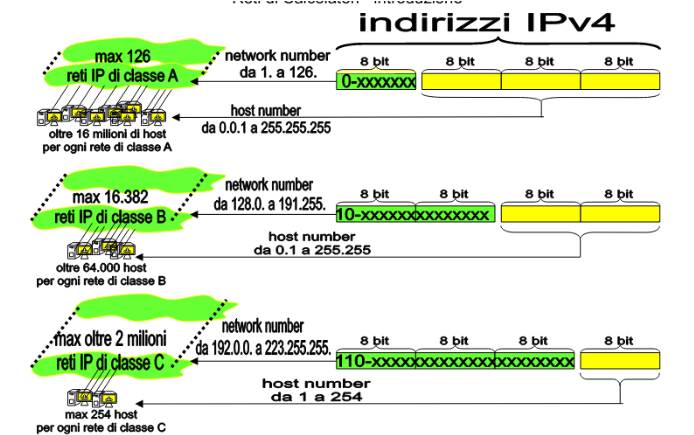
\includegraphics[width=10cm]{img/ipv4.png}
\end{center}

\subsection{Routing}
Il problema del \textbf{routing:} aggiornamento delle tabelle di forwarding dei router
\begin{itemize}
    \item Modifiche dei cammini per i dati nella rete
    \begin{itemize}
        \item Possibili soprattutto in rete senza fili a causa della mobilit\'a degli host
        \item Causate da modifiche agli accordi di servizio tra gestori di stistemi autonomi (AS)
    \end{itemize}
    \item Le modifiche dei cammini rendono sbagliate le tabelle di forwarding dei router
    \begin{itemize}
        \item I pacchetti possono andare perduti, o seguire strade diverse e arrivare disordinati
    \end{itemize}
    \item Occorrono reazioni da parte dei router per scoprire nuovi cammini
    \begin{itemize}
        \item \textbf{Protocolli (algoritmi) di routing:}
        \begin{itemize}
            \item Invio richieste: qualcuno cnosce il modo per arrivare al destinatario?
            \item Aggiornamento della tabella di forwarding con il cammino migliore
        \end{itemize}
    \end{itemize}
    Esempio di algoritmi di routing su internet: Fouting Information Protocol (RIP), Open Shortest Path First (OSPF), Border Gateway protocol (BGP)
\end{itemize}

\subsection{Protocollo ICMP}
Internet Control Message Protocol (ICMP), protocollo dei \textbf{messaggi di controllo} su internet:
\begin{itemize}
    \item Uno standart per definire la comunicazione di informazioni utili alla gestione di internet
    \item ICMP \'e usata da host, router e gateway per scambiare informazioni di livello rete, usando pacchetti definiti con il protocollo IP
    \begin{itemize}
        \item Notifica di errori di configurazione e gestione dei cammini e collegamenti
        \begin{itemize}
            \item Rete di destinazione non raggiungibile
            \item Rete di destinazione sconosciuta 
            \item Host destinazione non raggiungibile
            \item Host destinazione sconosciuto
            \item Protocollo richiesto non disponibile
            \item Ricerca di un cammino alternativo per la destinazione
        \end{itemize}
    \end{itemize}
\end{itemize}

\textbf{Ping} (verifica di connessione tra due host) e \textbf{traceroute} (mostra sequenza di router attraversati) sono applicazioni basate su \textbf{ICMP}. 

\subsection{Protocollo ARP e RARP}
Quando un router riceve un pacchetto destinato a un indirizzo IP della propria sottorete, esso deve rpodurre un frame di livello MAC/LLC che riporti specificato l'indirizzo MAC del destinatario, per poterlo passare al livello MAC/LLC per la trasmissione sulla rete locale.
\begin{itemize}
  \item Protocollo \textbf{Address Resolution Protocol (ARP)} 
\begin{itemize}
  \item Usato se il router non conosce l'indirizzo MAC corrispondente all'indirizzo IP
  \item Il router genera un frame spedito a tutti i dispositivi della rete locale dove si chiede: qual'è l'indirizzo MAC del dispositivo che ha questo indirizzo IP
  \item Se tale dispositivo esiste, esso risponde con un frame di livello MAC indirizzato al router nel quale viene evidenziato l'indirizzo MAC richiesto
\end{itemize}
\item Protocollo Reverse-ARP(\textbf{RARP})
\begin{itemize}
  \item E' la versione opposto del protocollo ARP, ma funziona allo stesso modo
  \item La domanda è: quale indirizzo IP corrisponde al dispositivo con questo indirizzo MAC?
\end{itemize}
\end{itemize}
\begin{center}
  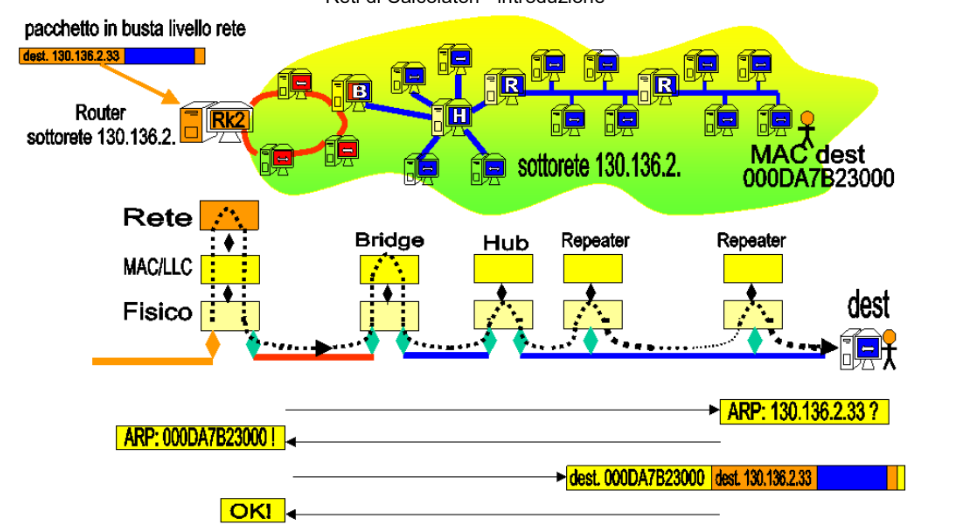
\includegraphics[width=10cm]{img/arp.png}
\end{center}
\subsection{Assegnazione indirizzi IP: DHCP}
Assegnazione automatica da parte di un server \textbf{Dynamic Host COnfiguration Protocol (DHCP)}: indirizzi IP dinamici:
\begin{itemize}
    \item Metodo automatico usato in reti wireless, reti locali e connessioni domestiche
    \item \textbf{Server DHCP}: è un host che implementa il servizio di assegnazione dell'indirizzo IP agli host che ne fanno richiesta
    i\mte Un DHCP server dispone di un blocco di host number liberi per la sua rete
    \item DHCP server associa indirizzi IP a indirizzi MAC dei dispositivi che lo richiedono 
    \item I dispositivi devono scegliere di affidarsi al server DHCP (ottiene indirizzo IP automaticamente)
\end{itemize}
\subsection{IPv6 e tunnelling IPv4}
Dal 1990 è attiva la definizione è l'implementazione di una nuova versione del protocollo di indirizzamento IP: \textbf{IPv6}.
\begin{itemize}
    \item \textbf{Indirizzi IPv6:} estesi a $128$ bit ($16$ byte) anzichè i $32$ bit ($4$ byte) di IPv4
    \item Nuova struttura dei campi della busta dei pacchetti di livello rete (IP)
\end{itemize}
Per ora la sperimentazione IPv6 avviene su reti separate (router IPv6). Ci sono casi di integrazione tra IPv4 e IPv6 usando tecniche di \textbf{tunnelling}, cioè spedire pacchetti IPv6 in buste IPv4. Nella lettura di un IPv6 se troviamo i due punti \textbf{(:)} significa che bisogna sostituirli con $4$ zeri.
\begin{center}
    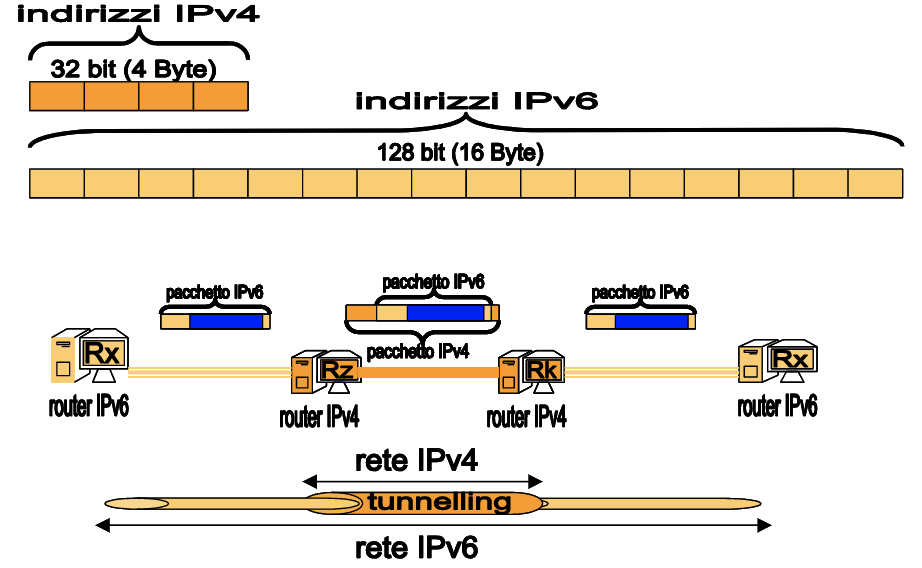
\includegraphics[width=8cm]{img/ipv6.png}
\end{center}
\newpage
\section{Livello trasporto}
I protocolli di Internet di quarto livello (trasporto) sono essenzialmente il \textbf{Trasmission Control Protocol (TCP)} e lo \textbf{User Data Protocol (UDP)}.
\begin{itemize}
    \item Livello trasporto: protocolli TCP e UDP
    \begin{itemize}
        \item Servizio \textbf{trasporto affidabile:} servizio di tipo connection-oriented
        \begin{itemize}
            \item configurazione de l\textbf{numero di porta} del \textbf{socket TCP}
            \item Numerazione sequenziale dei pacchetti, riordino, eliminazione duplicati
            \item Pacchetti di conferma della ricezione (acknowledgement di livello trasporto)
            \begin{itemize}
                \item Pacchetti non ricevuti spediti di nuovo
            \end{itemize}
            gestione della congestione e controllo di flusso dei pacchetti
            \begin{itemize}
                \item Meccanismi a finestra scorrevole (sliding window)
            \end{itemize}
        \end{itemize}
        \item Servizio \textbf{trasporto non affidabile} (protocollo UDP): servizio connectionless
    \end{itemize}
\end{itemize}
\begin{center}
    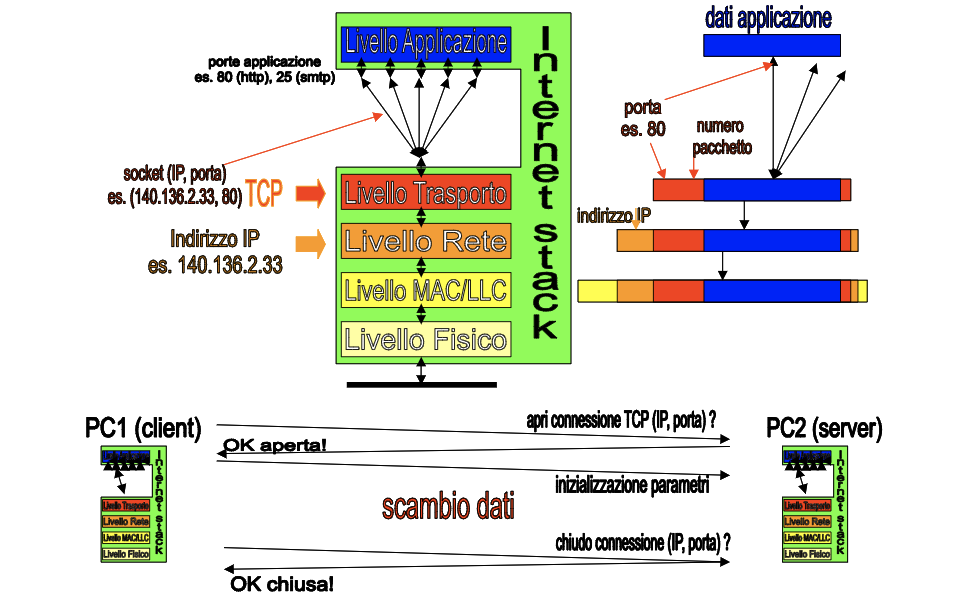
\includegraphics[width=6tcm]{img/trasporto.png}
\end{center}
\subsection{Livello trasporto su Internet: TCP}
TCP è il protocollo di livello trasporto usato di fatto su internet. Lo standard architetturale usato su Internet provede il \textbf{connubio TCP/IP}. TCP consente lo smistamento dei pacchett iverso le rispettive applicazioni in ascolto su porte.\\
TCP richiede \textbf{attivazione della connessione} punto a punto tra due socket. Il \textbf{socket} è formato da:
\begin{itemize}
    \item Indirizzo IP
    \item Numero di porta
\end{itemize}
In questo modo mette in comunicazione le applicazioni in attesa sui socket.\\
\textbf{Esempio:}\\
PC1(client) invia richiesta TCP di connessione sul socket del PC2 (server), se il socket esiste e non è occupato, TCP di PC2 risponde ok! Se riceve l'ok da PC2, TCP di PC1 può inviare i dati di configurazione. Ora avviene lo scambio dati veri e propri a livello TCP.\\\\
Una volta \textbf{rilasciata la connessione} si liberano le porte usate.
\begin{center}
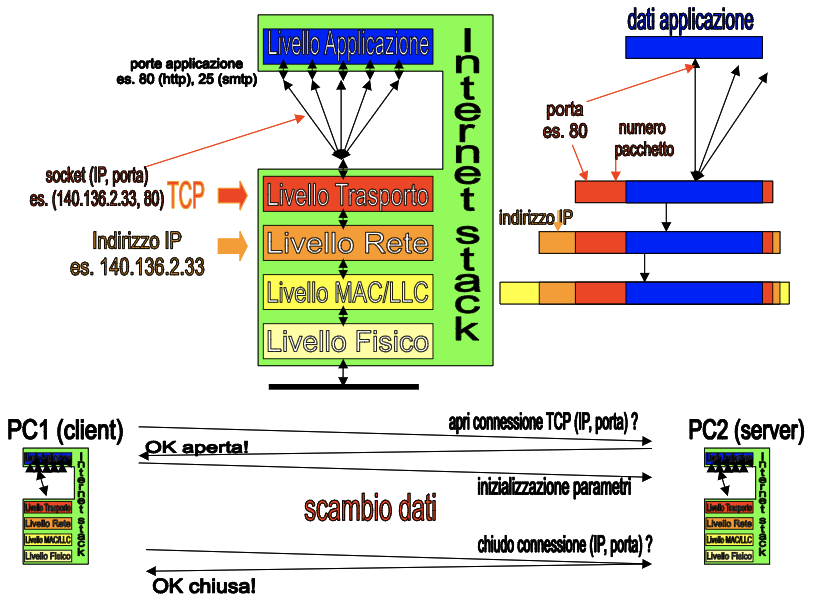
\includegraphics[width=7cm]{img/connessione.png}
\end{center}
\subsection{Controllo di flusso e congestione di rete}
TCP funziona tra due dispositivi di una rete, anche molto distanti tra loro, ed implementa tecniche di controllo di flusso e controllo della congestione di rete. Lo scopo del:
\begin{itemize}
    \item \textbf{Controllo di flusso} è inviare pacchetti al massimo ritmo sostenibile dal destinatario finale.
    \item \textbf{Controllo di congestione} è inviare pacchetti al massimo ritmo sostenibile dal router più lento della rete del mittente al destinatario finale
\end{itemize}
Esistono vari metodi: meccanismo a \textbf{finestra scorrevole (sliding window, SW)}
\begin{center}
    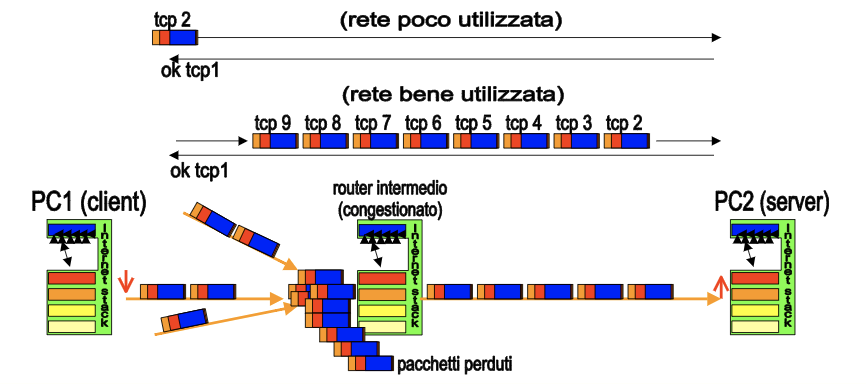
\includegraphics[width=8cm]{img/congestione.png}
\end{center}

\subsection{Finestra scorrevole di TCP}
Una \textbf{finestra scorrevole (sliding window, SW)} è un valore intero e rappresenta il \textbf{numero massimo di pacchetti} che un mittente può spedire di seguito, in attesa di ricevere la conferma. Ogni mittente TCP spedisce al massimo ritmo possibile un gruppo di SW pacchetti.
\begin{itemize}
    \item \textbf{Controllo di flusso:} non spedisce più di SW pacchetti oltre l'ultimo non confermato
    \begin{itemize}
        \item Se i primi SW pacchetti vengono confermati, spedisce i successivi SW pacchetti
        \item Se un pacchetto non viene confermato lo rispedisce, prima di spedire i successivi SW
    \end{itemize}
    \item \textbf{Controllo della congestione:} spedisce un numero SW variabile di pacchetti
    \begin{itemize}
        \item Se SW pacchetti spediti sono tutti confermati aumenta SW
        \item Appena un pacchetto degli SW inviati non viene confermato (scade il timeout) assumento che ciò sia dovuto a congestione su un router. Cerca di 
    \end{itemize}
\end{itemize}
\begin{center}
    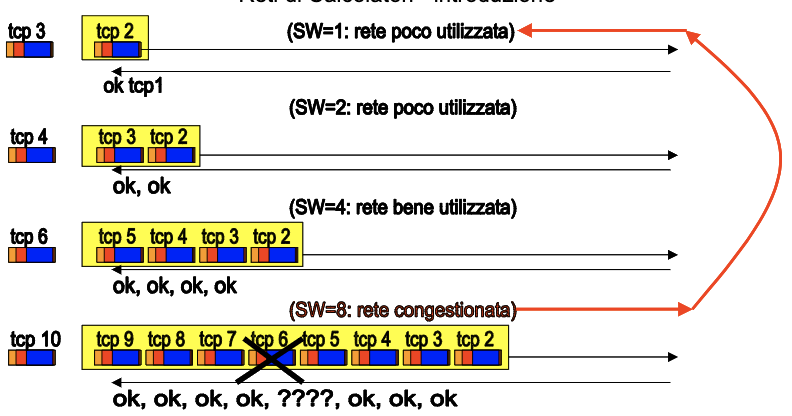
\includegraphics[width=6cm]{img/aumentoPacchetti.png}
\end{center}

\subsection{Nomi di dominio e servizio DNS}
Gli utenti preferiscono usare \textbf{nomi per le risorse in rete}, anziché IP. I nomi di dominio per le reti hanno una struttura \textbf{gerarchica}. Anche i nomi di dominio sono assegnati in modo univoco come i numeri di rete. I protocolli di rete e i router pretendono di usare indirizzi IP.\\
Il servizio \textbf{DNS (Domain Name System)}
\begin{itemize}
    \item E' basato su una catena di \textbf{server DNS} organizzati gerarchicamente
    \begin{itemize}
        \item Ogni host in rete deve conoscere almeno un DNS server
        \item Ogni server DNS conosce almeno un DNS server superiore
    \end{itemize}
    \item I server ricevono richieste e forniscono indirizzi IP
    \item Se un server non conosce la risposta inoltra la richiesta DNS a un server superiore
    \item I server DNS radice conoscono tutti i domini e i loro IP
\end{itemize}
\begin{center}
    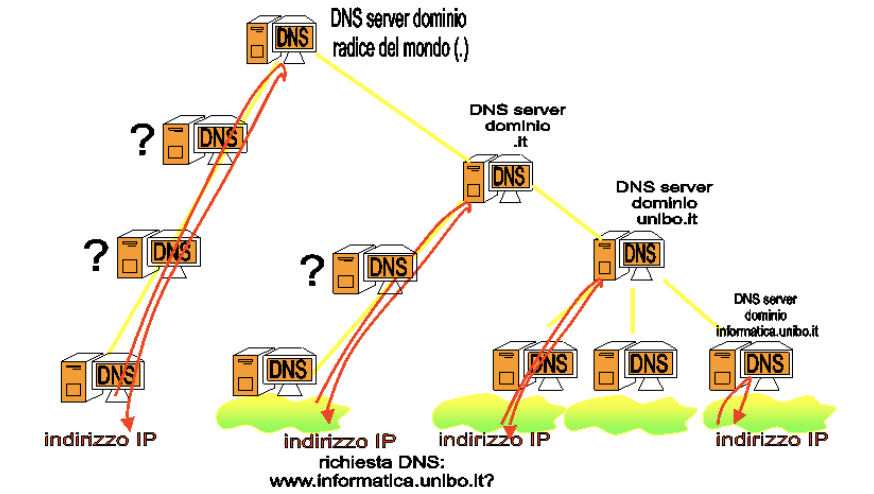
\includegraphics[width=6cm]{img/dns.png}
\end{center}

\section{Livello applicazione}

Il \textbf{livello applicazione:} primitive e protocolli per spedire e ricevere dati delle applicazioni. I livelli \textbf{sessione} e \textbf{presentazione} sono raramente implementati sugli host di internet. Il livello \textbf{applicazione} si appoggia sul livello trasporto. Esempi di famose applicazioni di rete sono:
\begin{itemize}
    \item \textbf{Posta elettronica:} basati su protocolli di livello applicazione:
    \begin{itemize}
        \item \textbf{SMTP}, per la spedizione e trasporto dei messaggi
        \item \textbf{POP3}, per la consegna dei messaggi all'utente
        \item \textbf{IMAP}, alternativa a POP3
    \end{itemize}
    \item \textbf{World Wide Web:} basato su applicazione e protocollo HTTP
    \begin{itemize}
        \item Hyper Text Trasfer Protocol (HTTP): protocollo per traasferire pagine web
    \end{itemize}
    \item \textbf{DNS:} Domain Name Service (protocollo DNS)
\end{itemize}
\begin{center}
    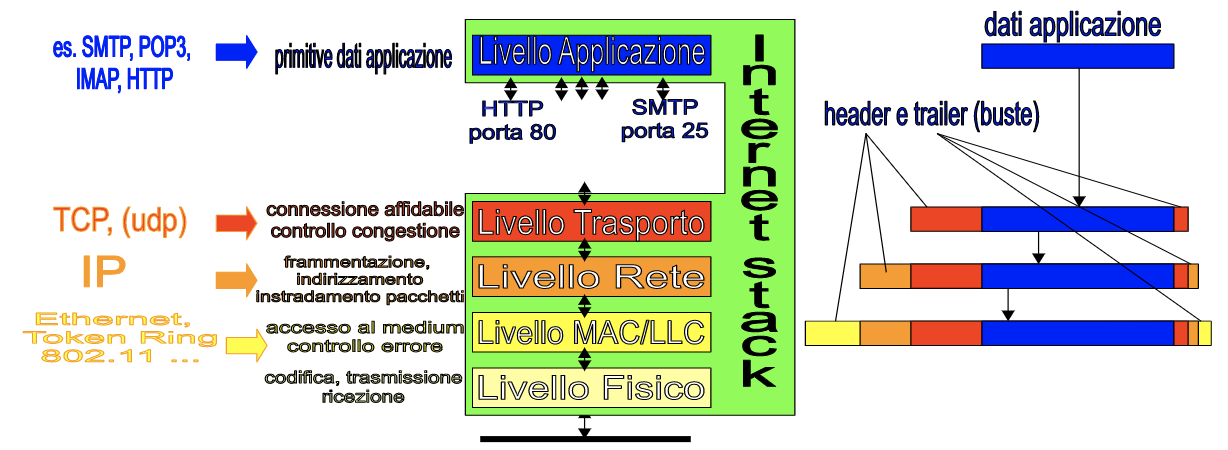
\includegraphics[width=7cm]{img/app.png}
\end{center}

\section{Network security}
La sicurezza di rete si basa su $4$ principi:
\begin{itemize}
    \item \textbf{Riservatezza}, solo chi invia e riceve devono capire il testo del messaggio
    \item \textbf{Autenticazione}, ognuno deve confermare la propria identità
    \item \textbf{Integrita dei messaggi}, i messaggi non devono arrivare alterati
    \item \textbf{Accesso e disponibilita}, il servizio deve essere disponibile agli utenti
\end{itemize}

Per rompere un sistema di \textbf{encriptazione} è necesario decriptare la chiave. Spesso viene adottato un metodo di \textbf{brute-force} dove vengono provate tutte le combinazioni possibili.
\begin{center}
    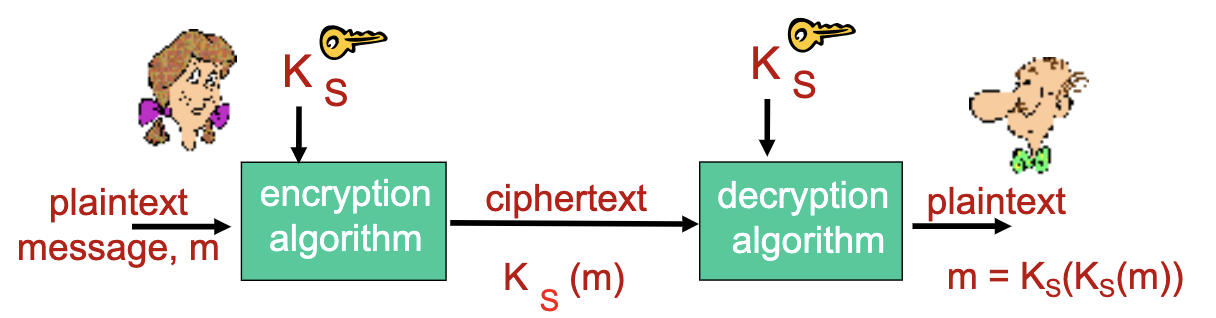
\includegraphics[width=7cm]{img/chiaviSimmetriche.png}
\end{center}
La crittografia \textbf{ simmetrica} è un metodo semplice per cifrare testo in chiaro dove la chiave di crittazione è la stessa chiave di decrittazione, rendendo l'algoritmo di cifratura molto performante e semplice da implementare.\\
Un semplice algoritmo di incriptazione è quello di \textbf{sostituzione}, dove andiamo a sostituire una lettera con un'altra. Un algoritmo più complesso invece è \textbf{DES} (Data Encryption Standard) che successivamente è stato decriptato. Successivamente nel 1999 venne \textbf{AES} (Avdanced Encryption Standard) che lavora su  blocchi da $128$ bit.\\ Viene adottato infine l'algoritmo \textb{RSA} (iniziali dei loro cognomi) che si basa sull'utilizzo di una chiave \textbf{pubblica} e \textbf{privata}.
Nel criptare i messaggi vengono utilizzate anche funzioni di \textbf{hash}, algoritmi comuni sono \textbf{MD5} che utilizza $128$-bit e \textbf{SHA-I} che ne utilizza $60$.
Il protocollo \textbf{SSL} Secure Layer Sockets, implementato nel 1994, una sua variazione è la \textbf{TLS} Transport Layer Security che vanno a creare un \textbf{tunnel} per criptare i dati.
\begin{center}
  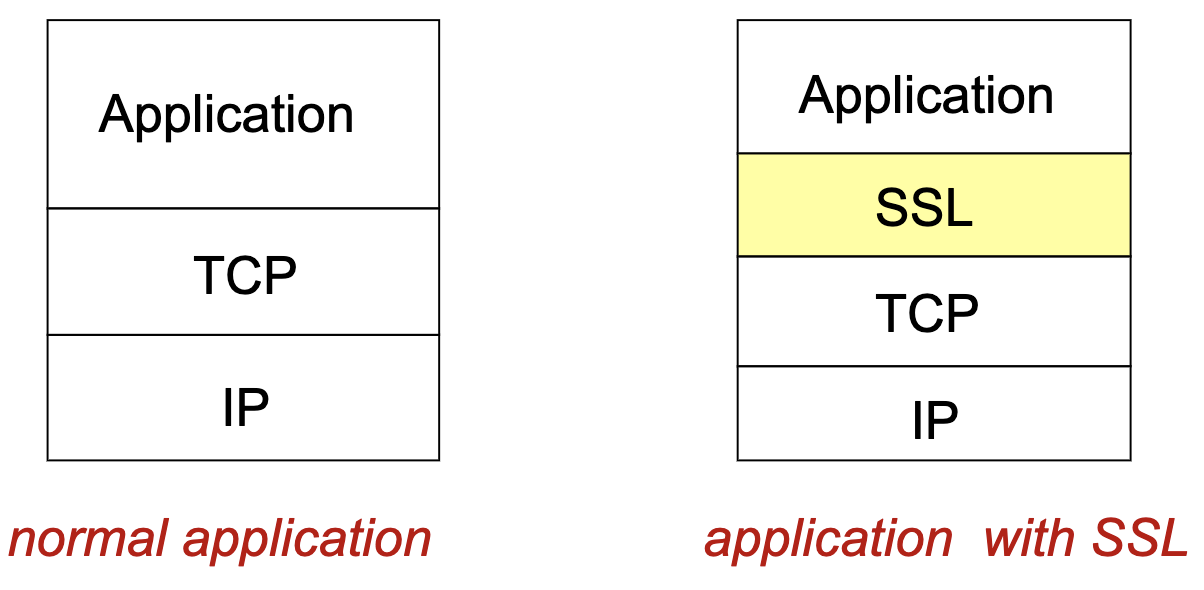
\includegraphics[width=5cm]{img/sslTcp.png}
\end{center}
Il protocollo SSL è composto da:
\begin{itemize}
  \item \textbf{Handshake}, dove vengono scambiati i certificati privati (criptatura della chiave)
  \item \textbf{Key derivation}, utilizzo dei certificati per decriptare i messaggi
  \item \textbf{Data transfer}, trasferimento dei dati in una serie di record
  \item \textbf{Connection closure}, messaggio per chiudere la connessione
\end{itemize}
Il \textbf{firewall} decide se bloccare o far passare informazioni a livello di rete.
Con lo \textbf{Stateless packet filter}: si permette di far viaggiare pacchetti senza una destinazione stabilita (connessione non aperta), al contrario dello \textbf{stateful packet filter}. L'\textbf{IDS: Intrusion Detection System} verifica le scansioni delle porte (port scanning) per verificare se si è possibilmente soggetti ad un attacco.
Un \textbf{protocollo} definisce il formato le regole e l'ordine del messaggio del mittente e del destinatario
La \textbf{network core} è il meccanismo di scambio dati tra i router. Una architettura \textbf{full duplex} consente la trasmissione e la ricezione dei dati, al contrario della \textbf{half duplex}, il quale ne permette solo una.

\section{Architetture di rete}
Esistono due possibili strutture di rete:
\begin{itemize}
  \item Client-server, dove abbiamo degli host sempre connessi con un proprio IP (\textbf{server}). Utile per avere dati centralizzati. \textbf{Client} utilizzati per comunicare con il server, non necessariamente in modo diretto e con un proprio IP anche dinamico
  \item peer-to-peer (P2P), non necessariamente dobbiamo avere dei server, e quindi possiamo avere una connessione diretta tra host. Questa tipologia è molto scalabile e permette lo scambio di indirizzi IP
\end{itemize}
Un \textbf{processo} è un programma che viene avviato senza un host. il \textbf{client process} è il processo che inizializza la comunicazione. Il \textbf{server process}, che aspetta la recezione della comunicazione.
Il \textbf{Socket}, permette lo scambio tra mittente e ricevente.
\begin{center}
  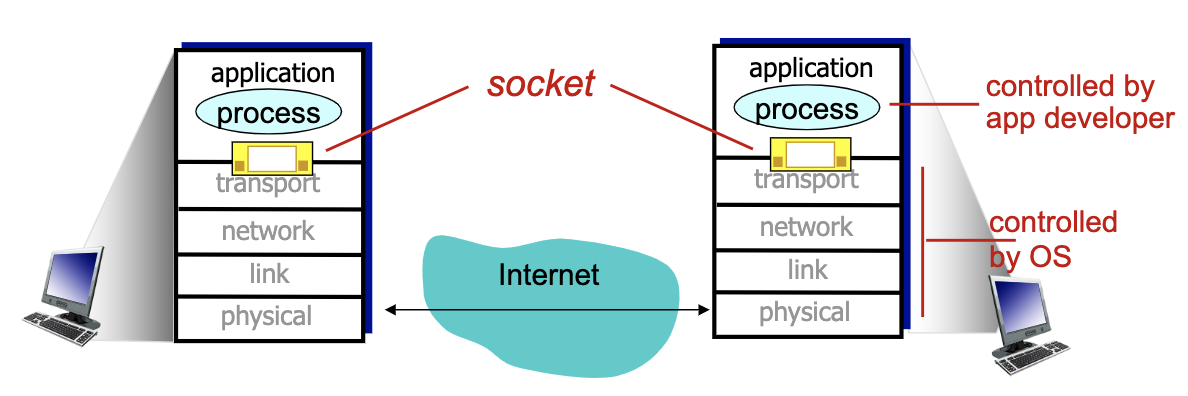
\includegraphics[width=6cm]{img/socket.png}
\end{center}
Per creare un socket abbiamo bisogno di un \textbf{protocollo} (https, udp, ecc.) e il numero di \textbf{porta} (80, 443, ecc.)
Per comprimere i dati di trasporto vengono utilizzati metodi \textbf{lossy} il quale abbrevia o elimina dati relativi al header della comunicazione tra host.
Http è \textbf{stateless}, cioè non mantiene informazioni riguardanti alle richieste del client passate.

\section{Domain Name System}

Il \textbf{DNS} traduce i nomi di dominio in indirizzi IP, in modo che i browser possano caricare le risorse Internet. Il DNS ha un hostname tradotto in un indirizzo IP e non è centralizzato.
Il DNS ha una struttura ad albero in cui troviamo:
\begin{itemize}
  \item \textbf{Root} DNS servers
  \item \textbf{Com} DNS servers
  \item \textbf{Org} DNS servers
\end{itemize}
\begin{center}
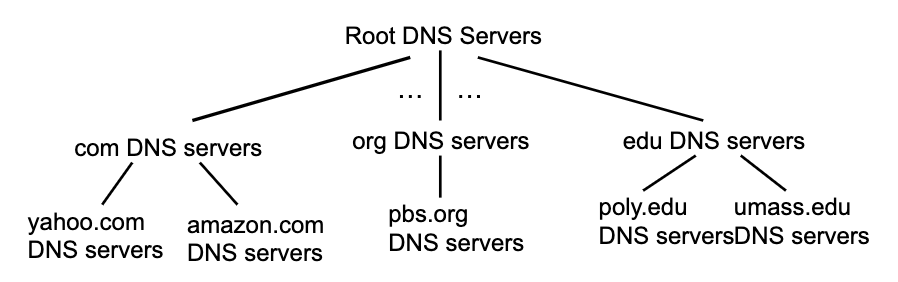
\includegraphics[width=6cm]{img/dnsScale.png}
\end{center}

I \textbf{top-level domain} (TLD) servers, sono responsabili della risoluzioni dei nomi del server.
Gli \textbf{Authoritative DNS server}, sono organizzazioni che fondano dei DNS server per mappare e indirizzare IP a siti web.\\
Ogni \textbf{ISP} (Internet Service Provider) ha un proprio DNS locale. Quando un host esegue una query DNS, esso la manda al proprio server locale.
\begin{center}
  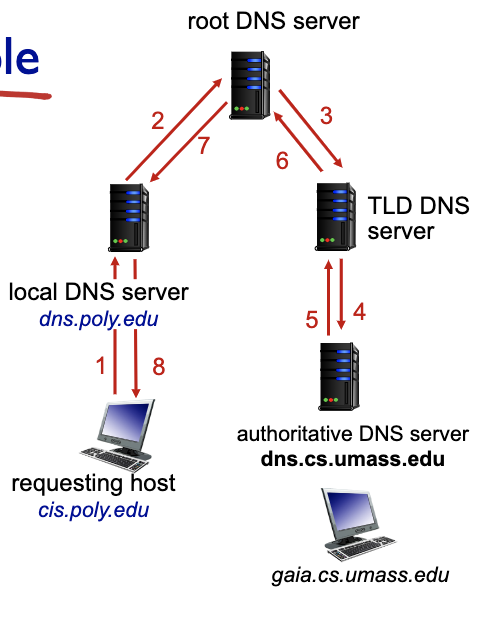
\includegraphics[width=6cm]{img/dnsResolution.png}
\end{center}
Il DNS esegue anche operazioni di \textbf{caching}. La memoria di cache va in timeout sparendo dopo un tempo definito (\textbf{TTL}).\\
Esistono diversi tipi di record DNS, i principali sono:
\begin{itemize}
  \item Record \textbf{A} il quale restituisce un indirizzo IPv4 a 32 bit, normalmente utilizzato per collegare un nome host al suo indirizzo IP.
  \item Record \textbf{CNAME}, permette di collegare un nome DNS ad un altro. La risoluzione continuerà con il nuovo nome indicato dal record CNAME. Come una sorta di \textbf{alias}
  \item Record \textbf{NS}, delega una zona DNS ad essere gestita da un server DNS autorevole per quel nome di dominio.
  \item Record \textbf{MX}, collega un nome di dominio ad una lista di server di posta autorevoli per quel dominio. I record indicano anche la preferenza di un server rispetto ad un altro.
\end{itemize}
\subsection{Peer to peer}
L'architettura \textbf{P2P} non è sempre attiva in server. Attraverso questa tecnica possiamo distribuire file, straming, VoIp. 
\begin{center}
  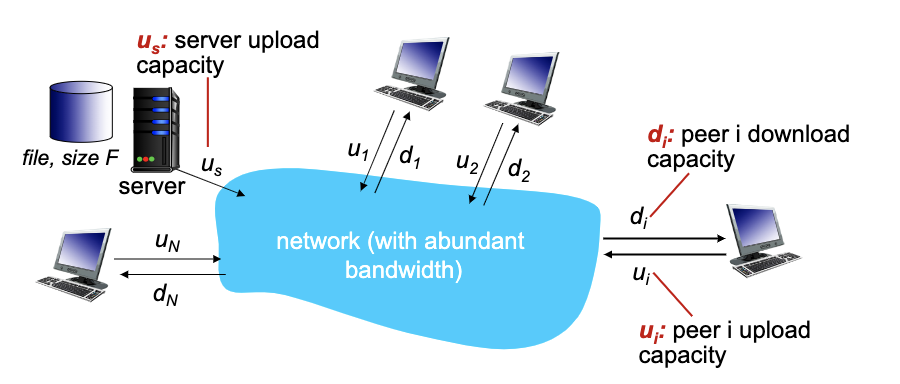
\includegraphics[width=6cm]{img/p2p.png}
\end{center}
\begin{itemize}
  \item \textbf{CBR}: (constant bit rate)
  \item \textbf{VBR}: (variable bit rate)
\end{itemize}
\textbf{DASH} (Dynamic Adaptive Streaming over HTTP) permette di dividere un file video in \textbf{chunks}; il client in questo modo può periodicamente consultare il server per la recezione dei dati.
Il server utilizza un file \textit{manifest file}: per distinguere i diversi chunks

\subsection{Content Delivery Network}
La \textbf{CDN} è il meccanismo di salvare copie di contenuti in server differenti
\begin{center}
  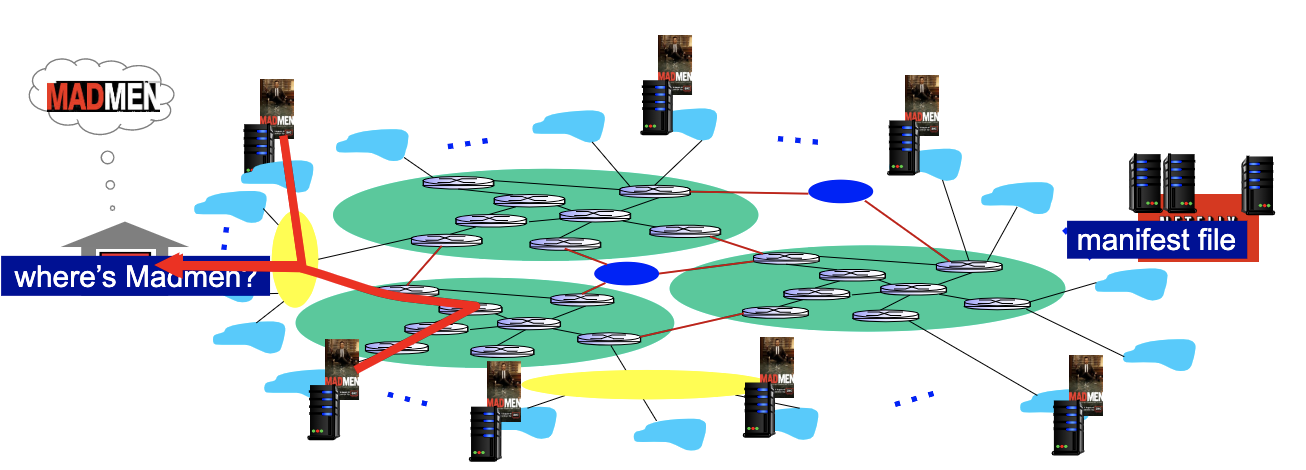
\includegraphics[width=6cm]{img/CDN.png}
\end{center}



\end{document}
